\documentclass{article}
\usepackage{amsmath}
\usepackage{mathtools}
\usepackage{gensymb}
\usepackage[a4paper,inner=1.5cm,outer=1.5cm,top=2cm,bottom=0.5cm]{geometry} 
\usepackage{xcolor}                    
\usepackage{tikz}                           
\usepackage{multicol}
\usepackage{pgfplots}
\usetikzlibrary{calc}
\usetikzlibrary{intersections}
\usetikzlibrary{intersections,calc,angles,quotes}
\usetikzlibrary{shapes,arrows,positioning,decorations.pathreplacing,calc}
\usetikzlibrary{calc,angles,positioning,intersections,quotes,decorations.markings}
\usepackage{tkz-euclide}
\usetikzlibrary{backgrounds}
\usetikzlibrary{calc,through}
\usetikzlibrary{angles}
\usetikzlibrary{fadings}
\usetikzlibrary{shapes.geometric}
\usetikzlibrary{shapes.symbols}
\usepackage{draftwatermark}
\usepackage{mathptmx}

\SetWatermarkText{\textcolor{black!30}{Mathema Shukur}}
\SetWatermarkFontSize{2 cm}
\usepackage[utf8]{inputenc}
\usepackage{fontspec}

\setmainfont{[Kalpurush.ttf]}
\newfontface{\en}{[Arial.ttf]} %%this is optional, if you want to use a secondary font. Any english font is supported
\newlength\Radius
\setlength\Radius{4cm}
\begin{document} 
	\Large
	\textcolor{red}{Welcome To} 
	\\
	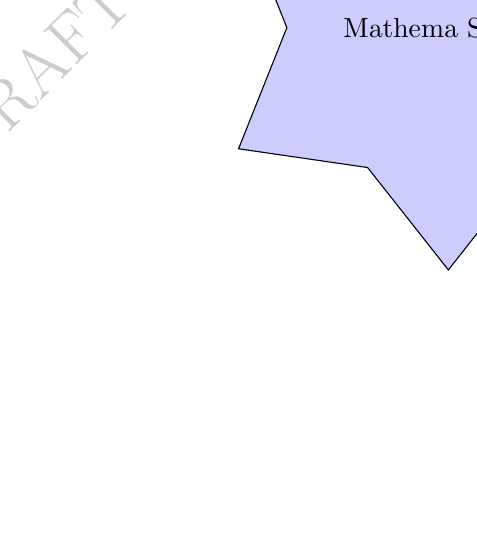
\begin{tikzpicture}
		\tikz \node [fill=blue!20,star,star points=6,draw] {Mathema Shukur };
	\end{tikzpicture}
	\\
	যাদের জন্যে প্রযোজ্যঃ  	\textcolor{magenta}{একাদশ ও দ্বাদশ শ্রেণীর শিক্ষার্থী} \\
	বিষয়ঃ \textcolor{magenta}{উচ্চতর গণিত ১ম পত্র} \\
	অধ্যায়ঃ \textcolor{magenta}{৩-সরলরেখা}\\ 
	Subtopicঃ  \textcolor{magenta}{ নির্ণায়কের  সাহায্যে ত্রিভুজের ক্ষেত্রফল  নির্ণয় করা area of triangle by determinant  }\\
	\\
	পূর্বজ্ঞানঃ\\ 
	Playlist: HSC-Matrix and Determinant\\
	টিউটোরিয়ালঃ ল্যাপলাস বিস্তার করে 3×3 নির্ণায়কের মান বের করা\\
	\\
	\begin{tikzpicture}[transform shape,scale=1]
		\draw [-latex,thick](-1,0) -- (10,0) node[right] {$x$} coordinate(x axis);
		\draw [-latex,thick](0,-1) -- (0,8) node[above] {$y$} coordinate(y axis);
		\fill[black] (0,0) circle (1.5 mm);
		\node at (-0.3,-0.3) {$\textcolor{purple}{O}$};	
		\fill[red] (3,5) circle (1 mm);
		\fill[red] (6,8) circle (1 mm);
		\fill[red] (8,4) circle (1 mm);
		\node at (2,5) {$\textcolor{red}{B(x_2,y_2)}$};	
		\node at (6,8.5) {$\textcolor{red}{A(x_1,y_1)}$};
		\node at (9.5,4) {$\textcolor{red}{C(x_3,y_3)}$};		
		\node at (3,-0.5) {$\textcolor{red}{L}$};		
			\node at (6,-0.5) {$\textcolor{red}{M}$};
				\node at (8,-0.5) {$\textcolor{red}{N}$};
		\draw[thick,magenta] (3,5)--(6,8);
			\draw[thick,magenta,dashed] (3,5)--(3,0);
		\draw[thick,magenta] (6,8)--(8,4);
			\draw[thick,magenta,dashed] (6,8)--(6,0);
		\draw[thick,magenta] (3,5)--(8,4);
			\draw[thick,magenta,dashed] (8,0)--(8,4);
	\end{tikzpicture}
	\\
		ট্রাপিজিয়ামের ক্ষেত্রফল \\
	\\ 
	$\frac{1}{2}\times $(ট্রাপিজিয়ামের সমান্তরাল বাহুদ্বয়ের যোগফল) $\times$ (ট্রাপিজিয়ামের সমান্তরাল বাহুদ্বয়ের মধ্যবর্তী দূরত্ব)\\ 
	\\ 
		\begin{tikzpicture}[transform shape,scale=1]
		\draw [-latex,thick](-1,0) -- (10,0) node[right] {$x$} coordinate(x axis);
		\draw [-latex,thick](0,-1) -- (0,8) node[above] {$y$} coordinate(y axis);
		\fill[black] (0,0) circle (1.5 mm);
		\node at (-0.3,-0.3) {$\textcolor{purple}{O}$};	
		\fill[red] (3,5) circle (1 mm);
		\fill[red] (6,8) circle (1 mm);
		\node at (2,5) {$\textcolor{red}{B(x_2,y_2)}$};	
		\node at (6,8.5) {$\textcolor{red}{A(x_1,y_1)}$};		
			\node at (9,4) {$\textcolor{blue}{T_{AB}=\frac{1}{2}(y_1+y_2)(x_1-x_2)}$};	
			\node at (3,-0.5) {$\textcolor{red}{L}$};		
			\node at (6,-0.5) {$\textcolor{red}{M}$};
				\node at (8,2) {$\textcolor{red}{LM=OM-OL}$};
					\node at (8,1) {$\textcolor{red}{LM=x_1-x_2}$};
		\draw[thick,magenta] (3,5)--(6,8);
		\draw[thick,magenta,dashed] (3,5)--(3,0);
		\draw[thick,magenta,dashed] (6,8)--(6,0);
	\end{tikzpicture}
\\
	\begin{tikzpicture}[transform shape,scale=1]
	\draw [-latex,thick](-1,0) -- (10,0) node[right] {$x$} coordinate(x axis);
	\draw [-latex,thick](0,-1) -- (0,8) node[above] {$y$} coordinate(y axis);
	\fill[black] (0,0) circle (1.5 mm);
	\node at (-0.3,-0.3) {$\textcolor{purple}{O}$};	
	\fill[red] (6,8) circle (1 mm);
	\fill[red] (8,4) circle (1 mm);
	\node at (6,8.5) {$\textcolor{red}{A(x_1,y_1)}$};
	\node at (9.5,4) {$\textcolor{red}{C(x_3,y_3)}$};
		\node at (3,4) {$\textcolor{blue}{T_{AC}=\frac{1}{2}(y_1+y_3)(x_3-x_1)}$};	
		\node at (6,-0.5) {$\textcolor{red}{M}$};
		\node at (8,-0.5) {$\textcolor{red}{N}$};	
			\node at (3,2) {$\textcolor{red}{MN=ON-OM}$};
		\node at (3,1) {$\textcolor{red}{MN=x_3-x_1}$};			
	\draw[thick,magenta] (6,8)--(8,4);
	\draw[thick,magenta,dashed] (6,8)--(6,0);
	\draw[thick,magenta,dashed] (8,0)--(8,4);
\end{tikzpicture}
\\
	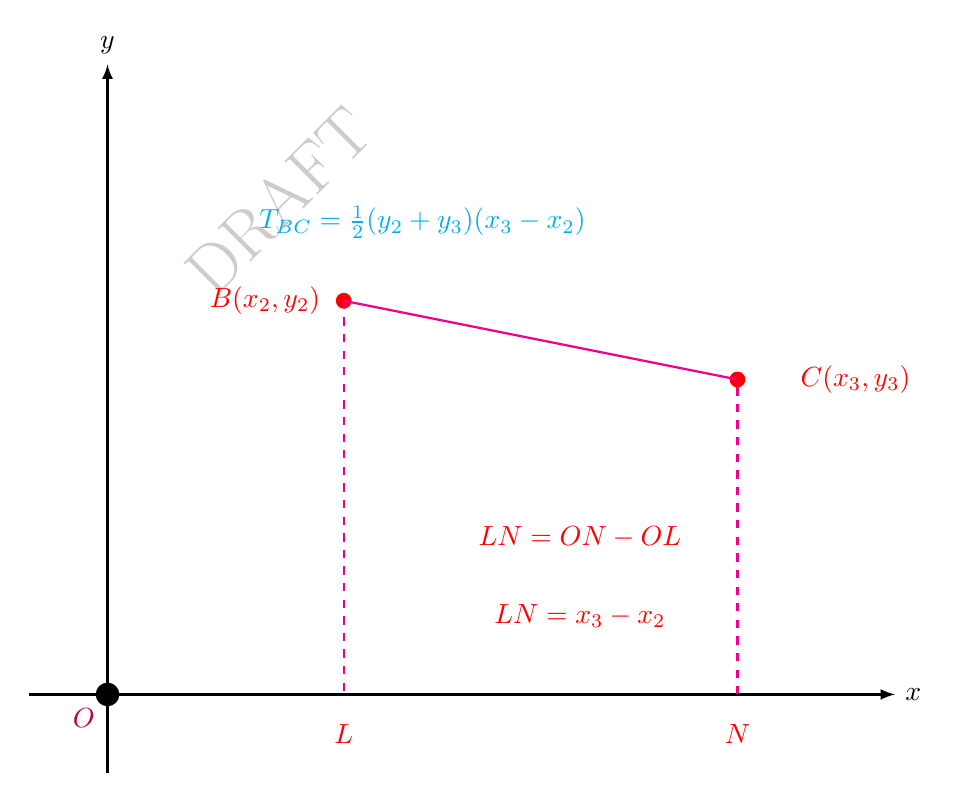
\begin{tikzpicture}[transform shape,scale=1]
	\draw [-latex,thick](-1,0) -- (10,0) node[right] {$x$} coordinate(x axis);
	\draw [-latex,thick](0,-1) -- (0,8) node[above] {$y$} coordinate(y axis);
	\fill[black] (0,0) circle (1.5 mm);
	\node at (-0.3,-0.3) {$\textcolor{purple}{O}$};	
	\fill[red] (3,5) circle (1 mm);
	\fill[red] (8,4) circle (1 mm);
	\node at (2,5) {$\textcolor{red}{B(x_2,y_2)}$};	
	\node at (9.5,4) {$\textcolor{red}{C(x_3,y_3)}$};		
		\node at (4,6) {$\textcolor{cyan}{T_{BC}=\frac{1}{2}(y_2+y_3)(x_3-x_2)}$};	
		\node at (3,-0.5) {$\textcolor{red}{L}$};		
		\node at (8,-0.5) {$\textcolor{red}{N}$};	
			\node at (6,2) {$\textcolor{red}{LN=ON-OL}$};
		\node at (6,1) {$\textcolor{red}{LN=x_3-x_2}$};		
	\draw[thick,magenta,dashed] (3,5)--(3,0);
	\draw[thick,magenta] (3,5)--(8,4);
	\draw[thick,magenta,dashed] (8,0)--(8,4);
\end{tikzpicture}
\\
	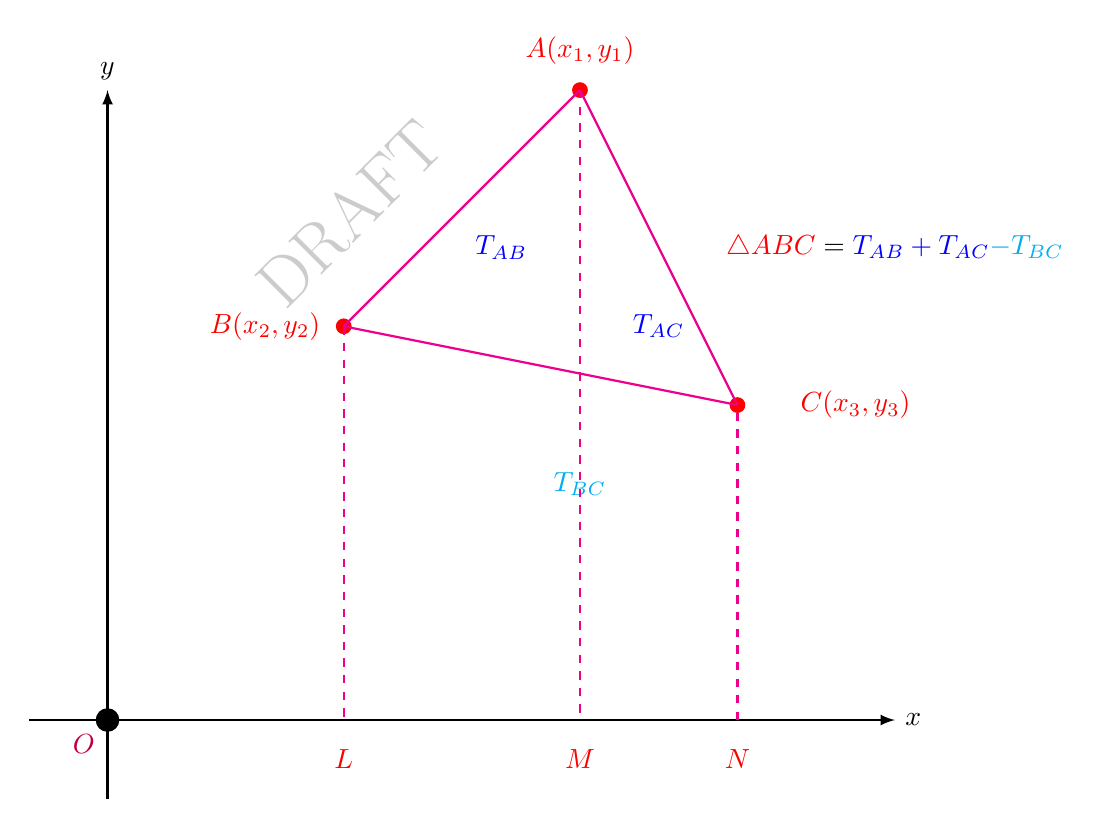
\begin{tikzpicture}[transform shape,scale=1]
	\draw [-latex,thick](-1,0) -- (10,0) node[right] {$x$} coordinate(x axis);
	\draw [-latex,thick](0,-1) -- (0,8) node[above] {$y$} coordinate(y axis);
	\fill[black] (0,0) circle (1.5 mm);
	\node at (-0.3,-0.3) {$\textcolor{purple}{O}$};	
	\fill[red] (3,5) circle (1 mm);
	\fill[red] (6,8) circle (1 mm);
	\fill[red] (8,4) circle (1 mm);
	\node at (6,3) {$\textcolor{cyan}{T_{BC}}$};		
		\node at (7,5) {$\textcolor{blue}{T_{AC}}$};	
			\node at (5,6) {$\textcolor{blue}{T_{AB}}$};	
	\node at (2,5) {$\textcolor{red}{B(x_2,y_2)}$};	
	\node at (6,8.5) {$\textcolor{red}{A(x_1,y_1)}$};
	\node at (9.5,4) {$\textcolor{red}{C(x_3,y_3)}$};	
		\node at (10,6) {$\textcolor{red}{\triangle ABC}=\textcolor{blue}{T_{AB}+T_{AC}}\textcolor{cyan}{-T_{BC}}$};		
			\node at (3,-0.5) {$\textcolor{red}{L}$};		
		\node at (6,-0.5) {$\textcolor{red}{M}$};
		\node at (8,-0.5) {$\textcolor{red}{N}$};	
	\draw[thick,magenta] (3,5)--(6,8);
	\draw[thick,magenta,dashed] (3,5)--(3,0);
	\draw[thick,magenta] (6,8)--(8,4);
	\draw[thick,magenta,dashed] (6,8)--(6,0);
	\draw[thick,magenta] (3,5)--(8,4);
	\draw[thick,magenta,dashed] (8,0)--(8,4);
\end{tikzpicture}
\\
\begin{align*}
\textcolor{red}{\triangle ABC}&=\textcolor{blue}{T_{AB}+T_{AC}}\textcolor{cyan}{-T_{BC}}\\
\\
&=\frac{1}{2}(y_1+y_2)(x_1-x_2)+\frac{1}{2}(y_1+y_3)(x_3-x_1)-\frac{1}{2}(y_2+y_3)(x_3-x_2)\\
\\
&=\frac{1}{2}\left[(y_1+y_2)(x_1-x_2)+(y_1+y_3)(x_3-x_1)-(y_2+y_3)(x_3-x_2)\right]\\
\\
&=\frac{1}{2}\left[x_1\,y_1-x_2\,y_1+x_1\,y_2-x_2\,y_2+x_3\,y_1+x_3\,y_3-x_1\,y_1-x_1\,y_3-x_3\,y_2+x_2\,y_2-x_3\,y_3+x_2\,y_3\right]\\
\\
&=\frac{1}{2}\left[-x_2\,y_1+x_1\,y_2+x_3\,y_1-x_1\,y_3-x_3\,y_2+x_2\,y_3\right]\\
\\
&=\frac{1}{2}\left[x_1\,y_2-x_1\,y_3-x_2\,y_1+x_2\,y_3+x_3\,y_1-x_3\,y_2\right]\\
\\
&=\frac{1}{2}\left[x_1(y_2-y_3)-x_2(y_1-y_3)+x_3(y_1-y_2)\right]\\
\\
&=\frac{1}{2}\left\{x_1\begin{vmatrix}
	y_2 & 1\\
	y_3 & 1
\end{vmatrix}-x_2\begin{vmatrix}
	y_1 & 1\\
	y_3 & 1
\end{vmatrix}+x_3\begin{vmatrix}
	y_1 & 1\\
	y_2 & 1
\end{vmatrix}\right\}\\
\\
&=\frac{1}{2}\begin{vmatrix}
x_1 &	y_1 & 1\\
x_2 & y_2 & 1\\
x_3 & y_3 & 1
\end{vmatrix}
\end{align*}
\\
সকল বোর্ড-২০১৮\\ 
$A(-2,3)$,\quad  $B(-4,2)$,\quad এবং $C(8,6)$ শীর্ষ  বিশিষ্ট ত্রিভুজের ক্ষেত্রফল নির্ণয় কর \\ 
\\
$(x_1,y_1)=(-2,3)$,\quad $(x_2,y_2)=(-4,2)$,\quad $(x_3,y_3)=(8,6)$\\
\\ 
\begin{align*}
&\frac{1}{2}\begin{vmatrix}
	x_1 &	y_1 & 1\\
	x_2 & y_2 & 1\\
	x_3 & y_3 & 1
\end{vmatrix}\\
\\
&=\frac{1}{2}\begin{vmatrix}
	-2 & 3 & 1\\
	-4 & 2 & 1\\
	8 & 6 & 1
\end{vmatrix}\\
&\boxed{Expansion \quad by \quad  First \quad  Column}\\ 
&=\frac{1}{2}\left\{(-2)\begin{vmatrix}
	2 & 1\\
	6 & 1
\end{vmatrix}-(-4)\begin{vmatrix}
	3 & 1\\
	6 & 1
\end{vmatrix}+(8)\begin{vmatrix}
	3 & 1\\
	2 & 1
\end{vmatrix}\right\}\\
\\
&=\frac{1}{2}\left[(-2)(2-6)-(-4)(3-6)+8(3-2)\right]\\
\\
&=\frac{1}{2}\left[8-12+8\right]\\
\\
&=2
\end{align*}
সিলেট বোর্ড-২০১৪\\
একটি ত্রিভুজের শীর্ষ বিন্দুগুলি $A(x,y)$,\,\, $B(1,2)$ ও $C(2,1)$ এবং এর ক্ষেত্রফল $6$ বর্গ একক হলে দেখাও যে $x+y=15$\\
\\
$(x_1,y_1)=(x,y)$,\quad $(x_2,y_2)=(1,2)$,\quad $(x_3,y_3)=(2,1)$\\
\\ 
\begin{align*}
	&\frac{1}{2}\begin{vmatrix}
		x_1 &	y_1 & 1\\
		x_2 & y_2 & 1\\
		x_3 & y_3 & 1
	\end{vmatrix}\\
	\\
	&=\frac{1}{2}\begin{vmatrix}
		x & y & 1\\
		1 & 2 & 1\\
		2 & 1 & 1
	\end{vmatrix}\\
	&\boxed{Expansion \quad by \quad  First \quad  Column}\\ 
	&=\frac{1}{2}\left\{(x)\begin{vmatrix}
		2 & 1\\
		1 & 1
	\end{vmatrix}-(1)\begin{vmatrix}
		y & 1\\
		1 & 1
	\end{vmatrix}+(2)\begin{vmatrix}
		y & 1\\
		2 & 1
	\end{vmatrix}\right\}\\
	\\
	&=\frac{1}{2}\left[(x)(2-1)-(1)(y-1)+(2)(y-2)\right]\\
	\\
	&=\frac{1}{2}\left[x-y+1+2y-4\right]\\
	\\
	&=\frac{1}{2}\left[x+y-3\right]\\
\end{align*}
\\
ত্রিভুজের ক্ষেত্রফল $6$ বর্গ একক \\
\\ 
\begin{align*}
\frac{1}{2}\left[x+y-3\right]&=6\\
\\
x+y-3&=12\\
\\
x+y&=12+3\\
\\
x+y&=15
\end{align*}
\end{document}